\begin{frame}{General Background}
\begin{columns}
\begin{column}{.48\linewidth}
\begin{block}{\visible<4->{Pressure on resources management}}
\begin{itemize}
    \visible<1->{\item Growing urbanisation}
    \visible<2->{\item Economical crises}
    \visible<3->{\item Environmental crises}
\end{itemize}
\end{block}
\end{column}
\begin{column}{.48\linewidth}
\visible<6->{
\begin{block}{\visible<6->{Contributions of ICT}}
\begin{itemize}
    \visible<7->{\item Changes in multiple level}
    \visible<8->{\item Digitalization}
    \visible<9->{\item Importance of information}
\end{itemize}
\end{block}
}
\end{column}
\end{columns}
\vspace{.3cm}
\visible<5->{
\begin{figure}
\centering
	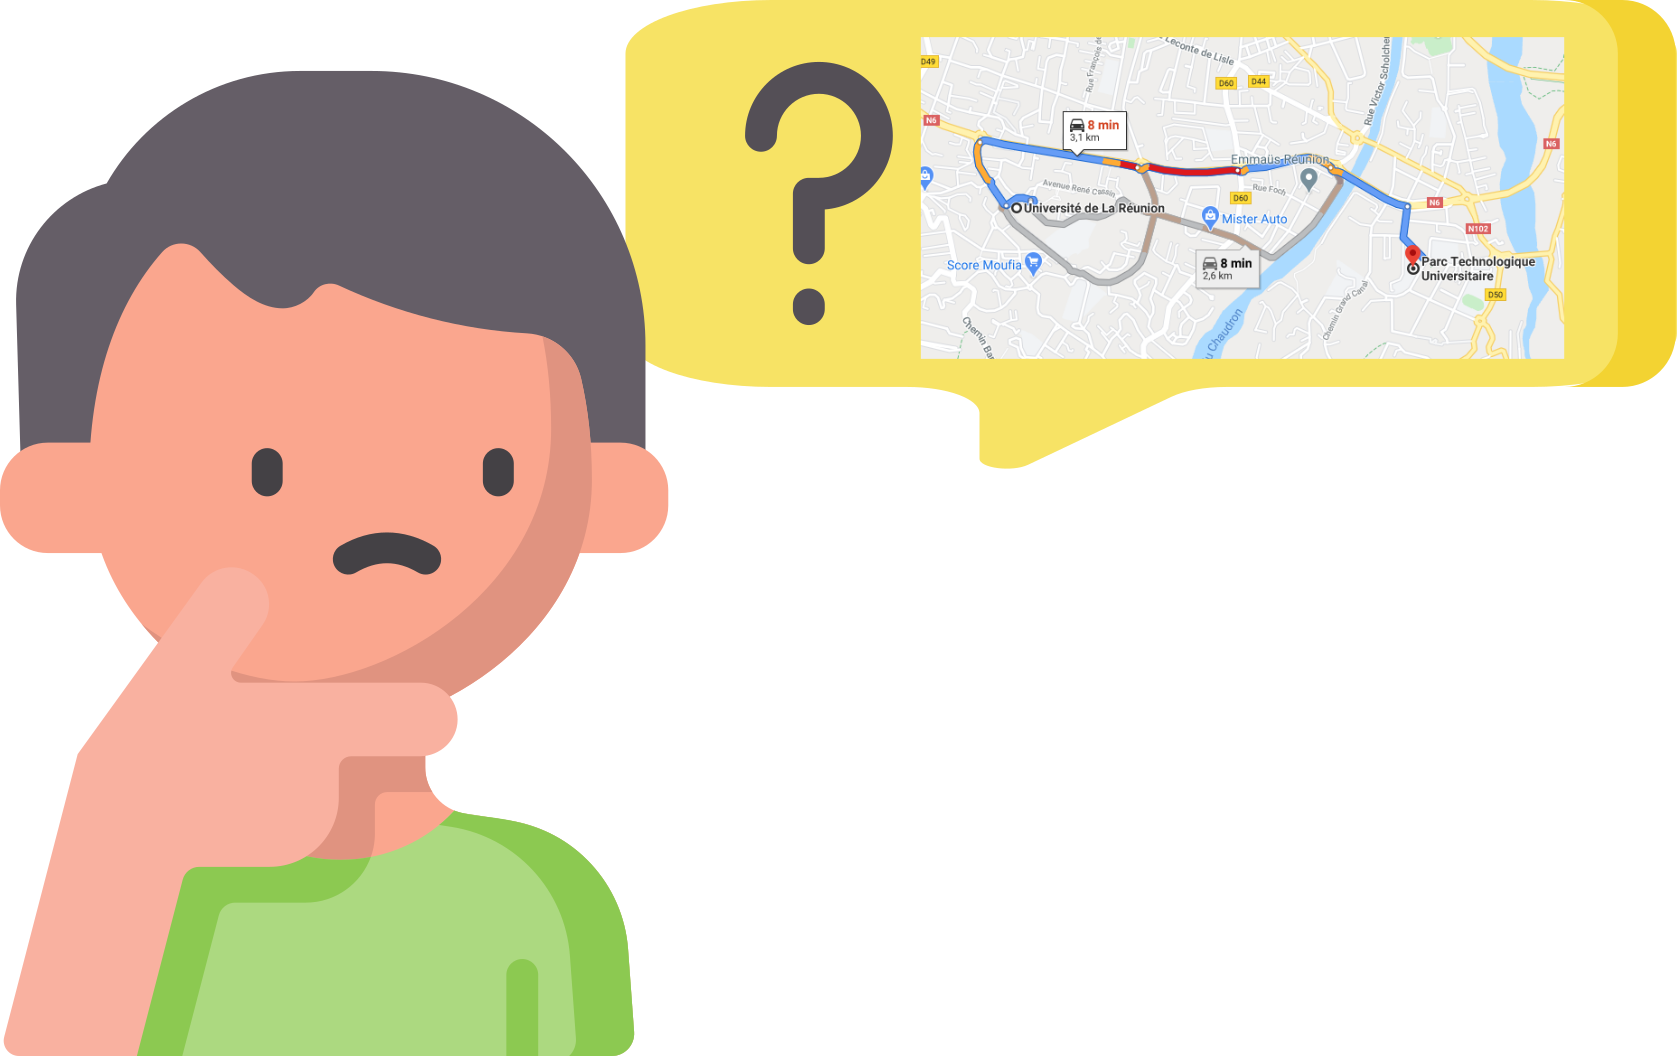
\includegraphics[width=.2\textwidth]{figures/question.png}
\end{figure}
}
\vspace{.3cm}
\centering \visible<10->{\alert{\huge{SMART CITY}}}
\note{
Nous faisons face à un phénomène d'urbanisation croissante accompagné de différentes crises économiques et environnementales qui engendrent d'autres crises comme la crise sanitaire que nous affrontons actuellement. Ces crises mettent une énorme pression sur la structure des villes et sur la gestion des ressources. Nous sommes alors contraints à chercher des solutions pratiques, techniques à ces différents problèmes, tout en prêtant uneattention particulière à l’environnement et au développement durable. En parallèle à cela, nous assistons, depuis ces dernières décennies à la montée en puissance des TIC qui contribue fortement à de grands changements au niveau de la ville, sur tous ses aspects : économique, culturel, transport, communication, etc. Les villes deviennent de plus en plus numériques et basées sur l’information.  Ces tendances ont conduit à la popularité du concept de ville intelligente ou smart city qui est considéré comme une solution aux problèmes évoquées précédemment.}
\end{frame}

%%%%%%%%%%%%%%%%%%%%%%%%%%%%%%%%%%%%%%%%%%%%%%%%%%%%%%%%%%%%%%%%%
\begin{frame}{General Background}{Smart City}
\begin{columns}
\begin{column}[l]{.48\linewidth}
\begin{figure}
	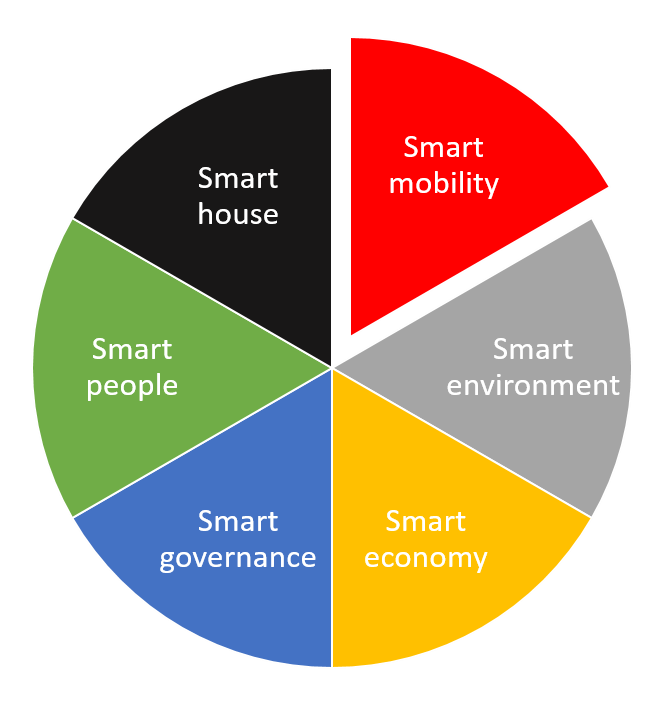
\includegraphics[width=\textwidth]{figures/smart_city.png}
\end{figure}
\end{column}
\begin{column}{.48\linewidth}
\visible<2->{\begin{block}{Criteria}
\begin{itemize}
    \item A bottom-up approach
    \item A more inclusive approach to citizens
    \item A participatory intelligence that emerges from the interactions between citizens and the system
\end{itemize}
\medbreak
\centering
\visible<3->{\alert{MULTI-AGENT SIMULATION}}
\end{block}}
\end{column}
\end{columns}
\note{\only<1>{Il n'existe pas encore de standard permettant de définir ce qu'est une ville intelligente. Plusieurs définitions peuvent se retrouver dans la littérature, mettant en valeur une ou plusieurs aspects de la ville. Celle que nous pensons la plus complète est celle de Giffinger. Giffinger défini une ville intelligente comme une ville qui est performante en 6 caractéristiques : l'environnement, l'économie, la mobilité, l'habitat, la gouvernance et le citoyen. Nous nous intéressons particulièrement à la mobilité intelligente. Cependant, nous pensons que nos solutions sont assez génériques pour être applicable aux autres domaines. Je reviendrai plus en détail sur notre cadre applicatif autour de la mobilité intelligente plus tard.}

\only<2>{Contrairement à beaucoup d'autres définitions qui ont tendance à négliger la place du citoyen ou aux mieux à les prendre en compte de façon marginale: en tant que consommateurs, dont les habitudes sont scrutées et régentées par des systèmes techniques, nous pensons que les citoyens occupent une place centrale dans la mise en oeuvre d'une ville intelligente. L'intelligence dont il est sujet ici est notamment une forme d'intelligence collective qui émerge des interactions entre le citoyen et le système. Dans ce contexte, les nouveaux outils du numérique facilitent grandement la participation des citoyens à l'élaboration des politiques, à la planification, etc. Ces citoyens échangent des informations et adoptent des comportements qui tendent à satisfaire des objectifs collectifs.}

\only<3>{L'approche multi-agent est une approche prometteuse permettant de modéliser ces types de systèmes. C'est une approche ascendante. Elle fait l'objet depuis longue date de recherches en intelligence artificielle distribuée. Appliqués au système de la ville, les sma permettent de décomposer cette dernière en plusieurs sous-ensembles plus simples, gérés par plusieurs entités autonomes, sociales, réactives et pro-actives appelées agents. Les sma permettent également de modéliser la non-linéarité et favorisent l’émergence des normes et des protocoles nécessaires pour les villes intelligentes.
\medbreak
Le domaine des sma mobilise des scientifiques issus majoritairement de l’informatique, des sciences cognitives et des systèmes complexes. Il produit un large spectre de solutions dans des champs d'applications tels que le développement de systèmes informatiques décentralisés, la résolution collective de problème, le développement de systèmes médiatisés ou encore la simulation de phénomènes complexes. C'est ce dernier champ d'application qui nous intéresse dans le cadre de nos travaux. Nous nous focalisons particulièrement sur les modèles de simulation multi-agent. Ces modèles de simulation servent à analyser le fonctionnement de scénario choisi, afin de déduire des enseignements pratiques de gestion opérationnelle dans le cadre de la conception et de la planification de villes intelligentes.}
}
\end{frame}

%%%%%%%%%%%%%%%%%%%%%%%%%%%%%%%%%%%%%%%%%%%%%%%%%%%%%%%%%%%%%%%%

\begin{frame}{Application Context}
\begin{itemize}
    \item Collective Adaptative System working group
    \item Multi-agent System :
    \begin{itemize}
        \item Focus on multi-agent simulation
        \item Hybrid approaches
    \end{itemize}
\end{itemize}


\note{
Cette thèse s’inscrit dans la continuité des travaux étudiés précédemment par le groupe de travail SCA du LIM. Notre équipe de recherche est spécialisée dans le paradigme des SMA, avec un accent particulier sur les aspects de simulations. Néanmoins, la politique actuelle de l’équipe s’oriente plus vers les approches de type hybrides. Cela veut dire qu’elle ne s’intéresse plus uniquement à la simulation, mais aussi à l’application dans un environnement réel. 
}
\end{frame}
%%%%%%%%%%%%%%%%%%%%%%%%%%%%%%%%%%%%%%%%%%
\begin{frame}{Application Context}
\begin{columns}
\begin{column}{.10\linewidth}
\begin{figure}
	
\includegraphics[width=\textwidth]{assets/icl.png}
\end{figure}
\begin{figure}
	
\includegraphics[width=\textwidth]{assets/saintDenis.png}
\end{figure}
\end{column}
\begin{column}[l]{.68\linewidth}
\begin{itemize}
    \item Multi-agent simulation of smart city and smart island : Smart mobility
    \item Multi-agent simulation of electric vehicle travel flows:
    \begin{itemize}
        \item SkuadCityModel
        \item SmartCityModel
    \end{itemize}
\end{itemize}
\vspace{1cm}
\textbf{Problem : } management of shared resources, limited in space and time
\end{column}
\end{columns}
\note{
Un des sous-thèmes développés consiste en l’application des simulations multi-agent dans le domaine des villes intelligentes et des îles intelligentes. Il s’agit d’un domaine en émergence dans notre équipe et sur lequel nous travaillons en collaboration avec des chercheurs de l'ICL et avec la mairie de Saint-Denis, La Réunion. Les problématiques abordées sont en lien avec la mobilité intelligente. Nous appliquons notre approche sur un modèle de simulation multi-agent de flux de déplacement de véhicules électriques sur un territoire que nous développons au sein même de notre équipe. Ce modèle s’appelle SkuadCityModel. Il se base sur un modèle développé par les chercheurs de l’ICL appelé SmartCityModel, sur lequel nous avons également contribué et qui a fait l'objet de deux contributions. Les problématiques abordées dans le cadre de cette thèse découlent des limites détectées lors de ces expérimentations. Nous nous intéressons notamment à des problématiques liées à la gestion de ressources partagées et limitées dans l’espace et dans le temps. Cette dernière fait partie des problèmes à l’origine même de la création du concept de ville intelligente. L’exemple sur lequel nous nous basons est celui du rechargement des véhicules électriques avec des bornes de recharge publiques.}
    
\end{frame}


%%%%%%%%%%%%%%%%%%%%%%%%%%%%%%%%%%%%%%%%%%
\begin{frame}{Application Context}{The example of the electric vehicle flow simulation}
\begin{columns}
\begin{column}{.48\linewidth}
\begin{figure}
	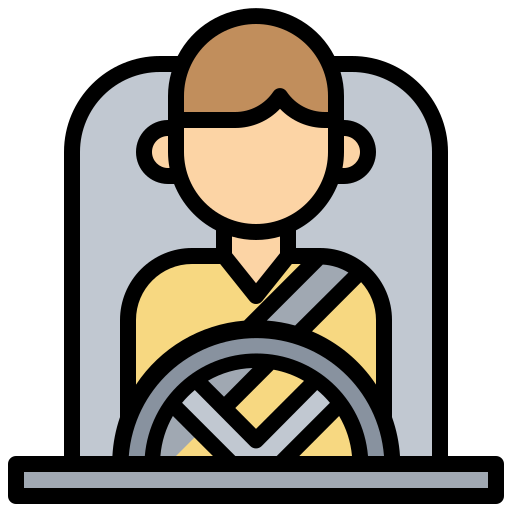
\includegraphics[width=.7\textwidth]{figures/driver.png}
\end{figure}
\centering {\Large Driver}
\end{column}
\begin{column}{.48\linewidth}
\begin{figure}
	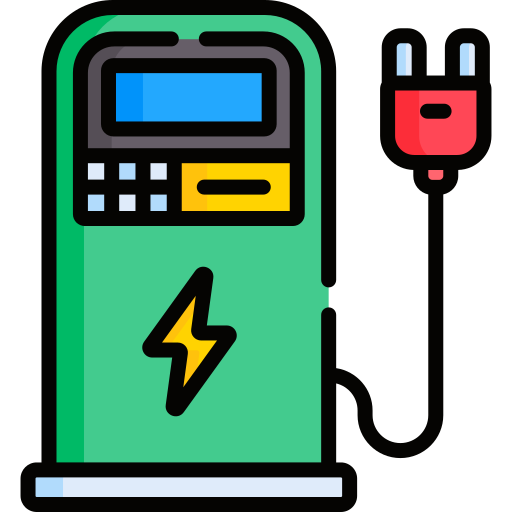
\includegraphics[width=.7\textwidth]{figures/electric-charge.png}
\end{figure}
\centering {\Large Charging point}
\end{column}
\end{columns}
\note{La recharge de véhicules électriques implique principalement deux entités : le conducteur de voiture électrique et la borne de recharge. Ces deux entités sont autonomes et indépendantes.}
\end{frame}


%%%%%%%%%%%%%%%%%%%%%%%%%%%%%%%%%%%%%%%%%%%%%%%%%%%%%%%%%%%%%%%%%%%%%%%%%%%%%%%
\begin{frame}{Application Context}{The example of the electric vehicle flow simulation}
\alt<1-6>{
\begin{block}{Driver}
\begin{columns}
\begin{column}{.18\linewidth}
\begin{figure}
	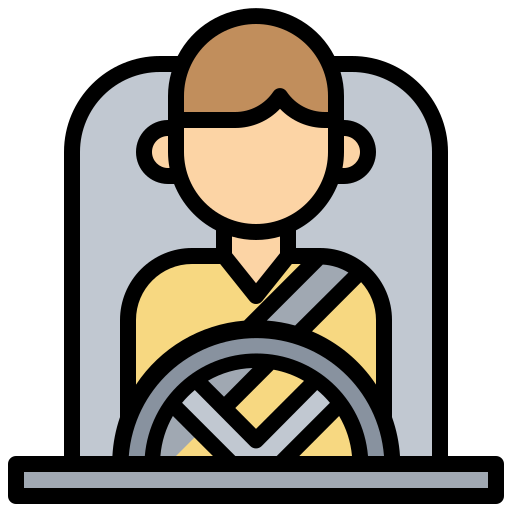
\includegraphics[width=\textwidth]{figures/driver.png}
\end{figure}
\end{column}
\begin{column}{.78\linewidth}
\begin{itemize}
    \visible<2->{\item Own a schedule composed of daily life activities that require travel}
    \visible<3->{\item The activities are situated in time and space}
    \visible<4->{\item \textbf{Main objective}: to accomplish all his planned activities}
    \visible<5->{\item \textbf{Main constraint}: recharging}
    \visible<6->{\item \textbf{Main strategy}: optimizing recharging
    \begin{itemize}
        \item Choosing the right time
        \item Minimise the recharging duration
    \end{itemize}
    
    }
\end{itemize}
\end{column}
\end{columns}
\end{block}
}{
\begin{block}{Charging point}
\begin{columns}
\begin{column}{.18\linewidth}
\begin{figure}
	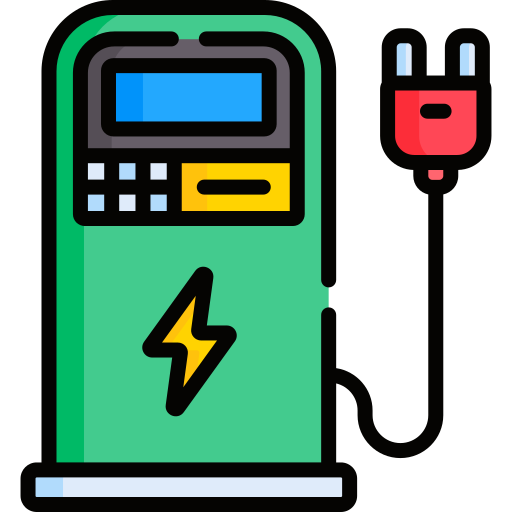
\includegraphics[width=\textwidth]{figures/electric-charge.png}
\end{figure}
\end{column}
\begin{column}{.78\linewidth}
\begin{itemize}
    \visible<7->{\item Limited number}
    \visible<8->{\item The availability is not guaranteed at any time or place}
    \visible<9->{\item \textbf{Main objective}: optimize its occupancy rate}
    \visible<10->{\item \textbf{Main constraint}: queue length}
    \visible<11->{\item \textbf{Main strategy}: optimize the distribution of electric vehicle recharging in its queue}
\end{itemize}
\end{column}
\end{columns}
\end{block}
}

\note{
\alt<1-6>{Dans SkuadCityModel, comme dans la réalité, un automobiliste possède un planning d'activité plus ou moins défini à l'avance. Ce planning se compose de différentes activités de la vie quotidienne nécessitant des déplacements : aller travailler, aller se divertir, rentrer chez soi ou faire ses courses. Ces activités sont situées dans le temps et dans l'espace. Cela revient à dire qu'à chaque activité, nous pouvons associer une composante spatiale (le conducteur va travailler à un endroit précis), et une composante temporelle (le conducteur part travailler à une heure précise).
\medbreak
L'objectif principal de l'automobiliste est d'accomplir l'ensemble des activités qu'il a prévues dans son planning. Pour ce faire, il se déplace en utilisant son véhicule électrique. Cependant, ce dernier possède une autonomie de batterie limitée. Par conséquent, le rechargement devient une contrainte. Le conducteur optimise alors au maximum le rechargement, de manière à ce qu'il puisse respecter son planning. Cette optimisation consiste à choisir le bon moment pour se recharger et à minimiser la durée du rechargement. Cette durée de rechargement inclut la durée d'attente au niveau de la borne de recharge.}
{
Le nombre de bornes de recharge est limité. En France par exemple, le ratio de véhicules par point de charge est de 5,7. Ce nombre peut varier en fonction de la situation géographique de la borne. Par conséquent, la disponibilité d'une borne n'est garantie ni à tout moment ni à tout endroit, car d'autres véhicules peuvent l'utiliser. Son objectif principal est d'optimiser son taux d'occupation. 
Cette situation a des répercussions tant au niveau de la borne qu'au niveau de l'automobiliste. Pour la borne, une forte demande de rechargement augmente le nombre de véhicules en attente (la longueur de la file d'attente). Elle est donc contrainte à trouver un moyen de bien gérer la répartition du rechargement des véhicules dans sa file d'attente. }
}
\end{frame}

\begin{frame}{Application Context}{The example of the electric vehicle flow simulation}
\textbf{Problem}: Management of a shared and limited resource in space and time.
\begin{itemize}
    \item lack of information for more precise reasoning.
    \item the charging point is not aware of the state of each vehicle or the schedule of the driver.
    \item no support is provided so that the driver can access all the information held by the charging point.
\end{itemize}

\note{ Ceci illustre donc un problème de gestion de ressources partagée et limitée dans l'espace et dans le temps.
\par La borne est contrainte à trouver un moyen de bien gérer la répartition du rechargement des véhicules dans sa file d'attente. Cependant, il s'agit d'une tâche difficile, car elle n'a connaissance ni de l'état de chaque véhicule ni du planning de l'automobiliste qui le conduit. Elle ne connaît donc pas la disponibilité de leur conducteur. Du côté de l'automobiliste, l'occupation des bornes et l'augmentation de la longueur de la file d'attente multiplient le temps nécessaire pour effectuer le rechargement. Elle réduit également le nombre de créneaux de rechargement disponibles. Cela constitue une contrainte qui pourrait perturber son planning et l'empêcher d'atteindre son objectif. L'automobiliste devra donc prendre en compte les informations concernant le planning et l'état de la borne dans ses décisions. Cependant, tout comme pour la borne, aucun support n'est prévu pour que l'automobiliste puisse accéder à la totalité des informations qui sont détenues par la borne.}
    
\end{frame}